\section*{Exercice 187 -- Circuit hydraulique}
\setcounter{exo}{0}


Le circuit hydraulique représenté sur la figure est composé de 6 modules :
\begin{itemize}
\item (a)	une pompe à engrenages entraînée par le moteur à gaz ;
\item (b)	un clapet anti-retour et une valve de décharge tarée pour s'enclencher à \SI{160}{bar} et se remettre en position fermée à \SI{100}{bar} ;
\item (c)	un accumulateur oléopneumatique de volume nominal \SI{1,4}{L} ;
\item (d)	un limiteur de pression ;
\item (e)	un servo-distributeur à effet proportionnel 4/3 à centre fermé ;
\item (f)	deux vérins simple effet, de diamètre \SI{32}{mm} pour chaque piston et de \SI{200}{mm} de course.
\end{itemize}

\begin{center}
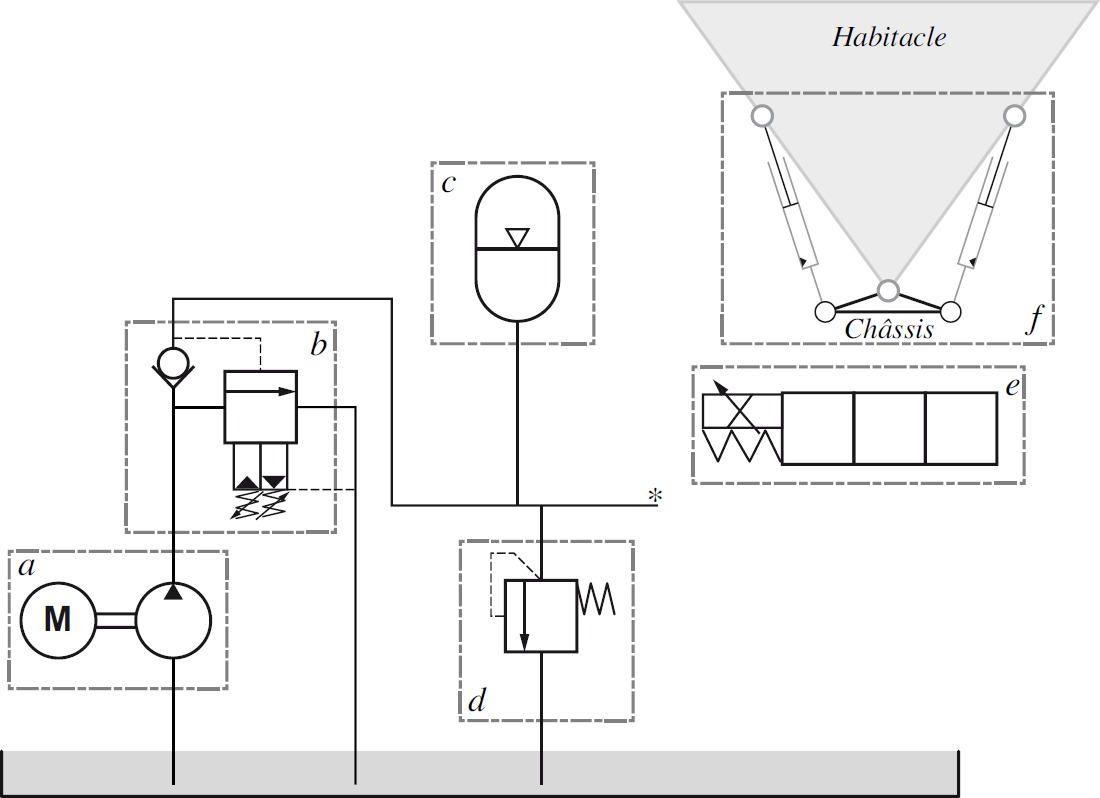
\includegraphics[width=\linewidth]{028_01}
\end{center}
\subparagraph{}\textit{Compléter le câblage du circuit hydraulique à partir du signe « * », ainsi que le schéma du servo-distributeur.}
\ifprof
\begin{corrige}
\end{corrige}
\else
\fi

Au démarrage du véhicule, la valve de décharge du module (b) est fermée. Le distributeur à effet proportionnel (e) est en position médiane, les vérins sont donc immobiles. La commande des vérins est initialement bloquée par une temporisation.

\subparagraph{}\textit{En considérant les conditions initiales évoquées, expliquer, en commençant à l'instant de démarrage de la pompe, le comportement du circuit hydraulique en précisant clairement les différentes phases de fonctionnement. Quelle est l'utilité de la temporisation ? }
\ifprof
\begin{corrige}
\end{corrige}
\else
\fi

\subparagraph{}\textit{On souhaite remplacer cette temporisation par un capteur. Préciser la grandeur qu'il devra mesurer. Donner un avantage et un inconvénient du remplacement de la temporisation par ce capteur.}
\ifprof
\begin{corrige}
\end{corrige}
\else
\fi
